% DataVo DBMS native PGFPlots figures.
% Exact coordinates are taken from whitepaper_benchmark_rerun_2026-07-03-v2.txt
% (the canonical rerun log; the SQLite fullfsync row is the retained macOS validation run).
% Preamble requirements:
% \usepackage{pgfplots}
% \usepackage{xcolor}
% \usepackage{graphicx}
% \pgfplotsset{compat=1.18}

\definecolor{datavoBlue}{HTML}{0072B2}
\definecolor{datavoGreen}{HTML}{009E73}
\definecolor{datavoDarkGreen}{HTML}{004D40}
\definecolor{datavoFreshGreen}{HTML}{2FBF71}
\definecolor{datavoLightBlue}{HTML}{56B4E9}
\definecolor{datavoTeal}{HTML}{0A9396}
\definecolor{sqliteOrange}{HTML}{E69F00}
\definecolor{sqliteRed}{HTML}{D55E00}
\definecolor{sqliteDarkRed}{HTML}{8B1E00}
\definecolor{liteDbPink}{HTML}{CC79A7}
\definecolor{neutralGray}{HTML}{7A869A}

% Figure 1: Disk CRUD WAL Log-Scale Time Comparison
\begin{center}
\resizebox{\linewidth}{!}{%
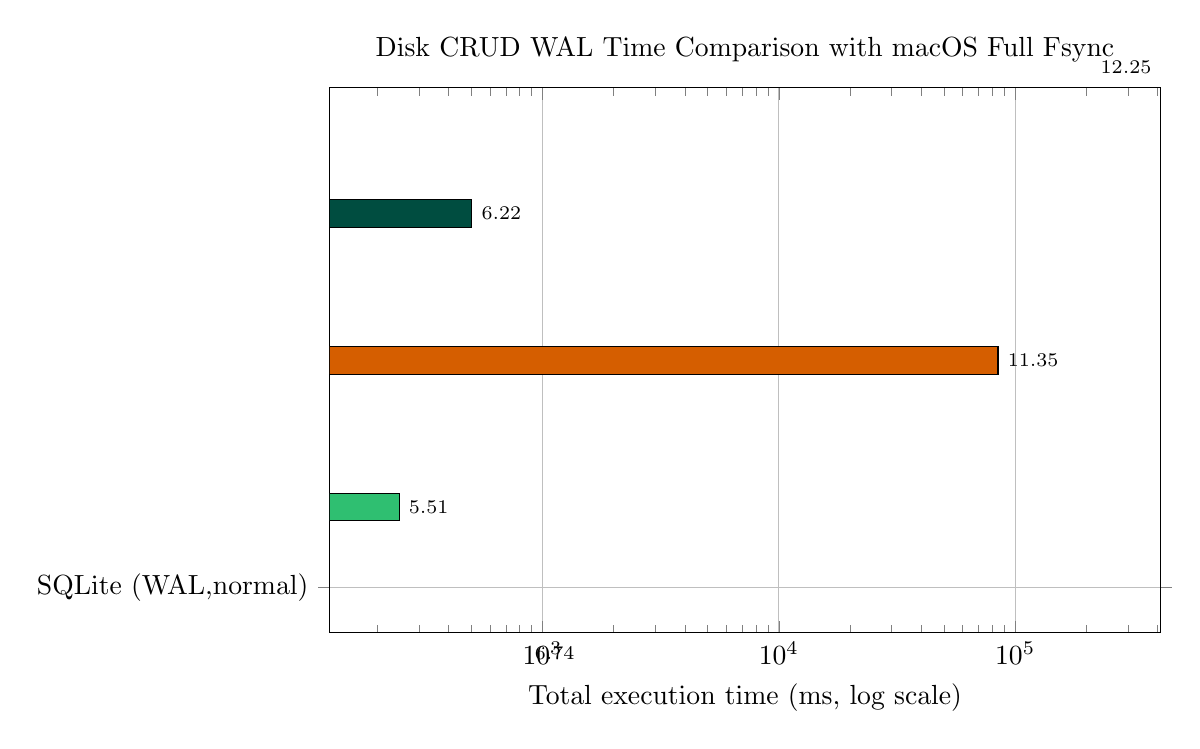
\begin{tikzpicture}
\begin{axis}[
    xbar,
    xmode=log,
    width=\linewidth,
    height=8.5cm,
    xlabel={Total execution time (ms, log scale)},
    symbolic y coords={
        {SQLite (WAL,normal)},
        {DataVo (LSM Relaxed)},
        {SQLite (WAL,full)},
        {DataVo (LSM Production)},
        {SQLite (WAL,full+fullfsync)}
    },
    ytick=data,
    nodes near coords,
    nodes near coords align={horizontal},
    every node near coord/.append style={font=\scriptsize},
    grid=major,
    title={Disk CRUD WAL Time Comparison with macOS Full Fsync},
]
\addplot[fill=sqliteOrange] coordinates {(842.914,{SQLite (WAL,normal)})};
\addplot[fill=datavoFreshGreen] coordinates {(247.080,{DataVo (LSM Relaxed)})};
\addplot[fill=sqliteRed] coordinates {(84638.110,{SQLite (WAL,full)})};
\addplot[fill=datavoDarkGreen] coordinates {(501.870,{DataVo (LSM Production)})};
\addplot[fill=sqliteDarkRed] coordinates {(209282.571,{SQLite (WAL,full+fullfsync)})};
\end{axis}
\end{tikzpicture}
}
\end{center}

% Figure 4: Thread Scaling OPS Curve
\begin{center}
\resizebox{0.9\linewidth}{!}{%
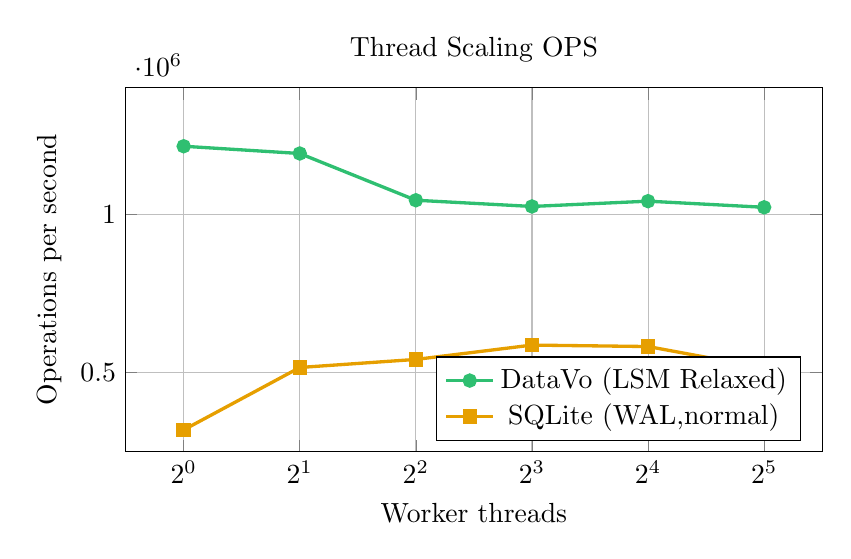
\begin{tikzpicture}
\begin{axis}[
    width=0.86\linewidth,
    height=6.2cm,
    xmode=log,
    log basis x=2,
    xtick={1,2,4,8,16,32},
    xlabel={Worker threads},
    ylabel={Operations per second},
    ymin=250000,
    ymax=1400000,
    yticklabel={\pgfmathprintnumber{\tick}},
    grid=major,
    legend pos=south east,
    title={Thread Scaling OPS},
]
\addplot[color=datavoFreshGreen, mark=*, line width=1.2pt] coordinates {
    (1,1215413.207)
    (2,1192483.021)
    (4,1044648.267)
    (8,1025016.936)
    (16,1041723.883)
    (32,1022364.692)
};
\addlegendentry{DataVo (LSM Relaxed)}
\addplot[color=sqliteOrange, mark=square*, line width=1.2pt] coordinates {
    (1,318474.934)
    (2,515803.275)
    (4,541284.774)
    (8,586604.721)
    (16,582041.070)
    (32,514214.285)
};
\addlegendentry{SQLite (WAL,normal)}
\end{axis}
\end{tikzpicture}
}
\end{center}

% Figure 4b: Strict-Durability Thread Scaling (WAL Group Commit)
\begin{center}
\resizebox{0.7\linewidth}{!}{%
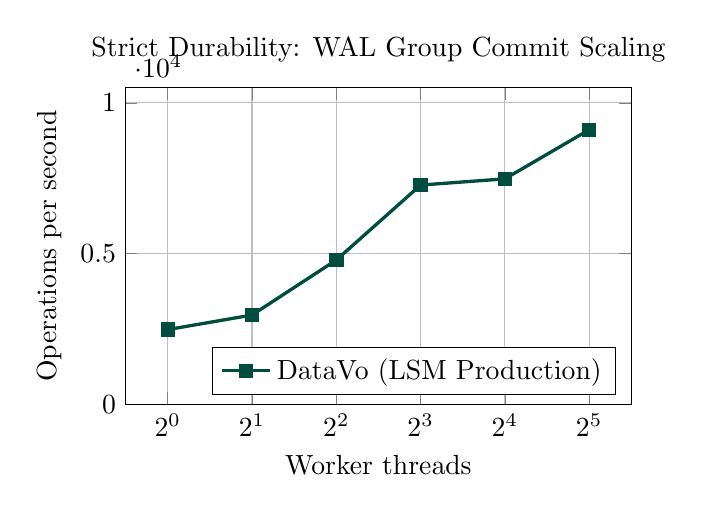
\begin{tikzpicture}
\begin{axis}[
    width=0.66\linewidth,
    height=5.6cm,
    xmode=log,
    log basis x=2,
    xtick={1,2,4,8,16,32},
    xlabel={Worker threads},
    ylabel={Operations per second},
    ymin=0,
    ymax=10500,
    yticklabel={\pgfmathprintnumber{\tick}},
    grid=major,
    legend pos=south east,
    title={Strict Durability: WAL Group Commit Scaling},
]
\addplot[color=datavoDarkGreen, mark=square*, line width=1.2pt] coordinates {
    (1,2478.648)
    (2,2962.324)
    (4,4788.347)
    (8,7274.764)
    (16,7480.346)
    (32,9110.373)
};
\addlegendentry{DataVo (LSM Production)}
\end{axis}
\end{tikzpicture}
}
\end{center}

% Figure 5: YCSB Mixed Write Tail
% Rerun metrics: DataVo (LSM Relaxed) = 626,690 OPS, read P99 0.000917 ms, write P99 1.333833 ms.
% SQLite (WAL,normal) read P99 = 0.010500 ms.
\begin{center}
\resizebox{0.86\linewidth}{!}{%
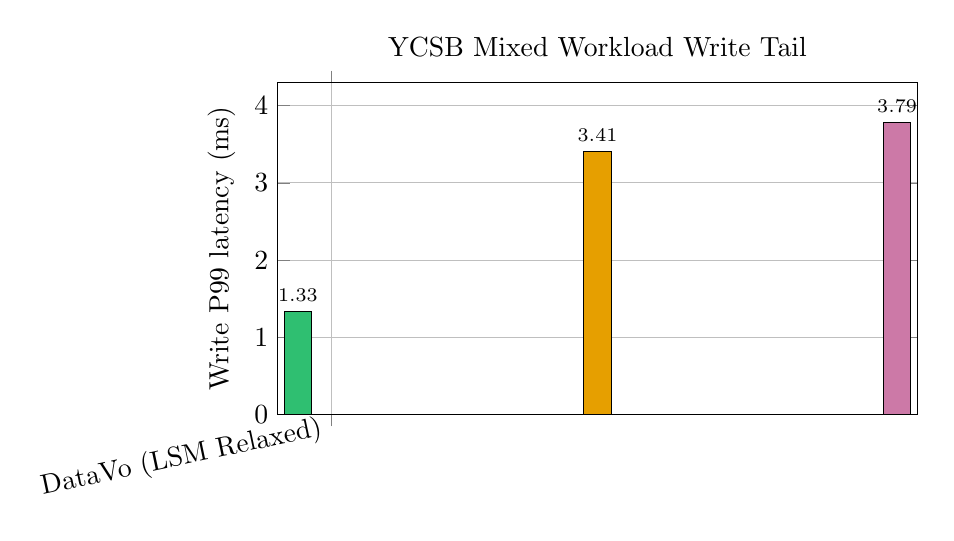
\begin{tikzpicture}
\begin{axis}[
    ybar,
    width=0.8\linewidth,
    height=5.8cm,
    ylabel={Write P99 latency (ms)},
    symbolic x coords={{DataVo (LSM Relaxed)},{SQLite (WAL,normal)},LiteDB},
    xtick=data,
    x tick label style={rotate=12, anchor=east},
    ymin=0,
    ymax=4.3,
    nodes near coords,
    nodes near coords align={vertical},
    every node near coord/.append style={font=\scriptsize},
    grid=major,
    title={YCSB Mixed Workload Write Tail},
]
\addplot[fill=datavoFreshGreen] coordinates {({DataVo (LSM Relaxed)},1.333833)};
\addplot[fill=sqliteOrange] coordinates {({SQLite (WAL,normal)},3.408333)};
\addplot[fill=liteDbPink] coordinates {(LiteDB,3.785125)};
\end{axis}
\end{tikzpicture}
}
\end{center}

% Figure 6: Space Amplification
% Rerun metrics: DataVo (LSM Relaxed) disk 66.443 MB, recovery 0.500 ms, GC 206.688 MB.
\begin{center}
\resizebox{0.86\linewidth}{!}{%
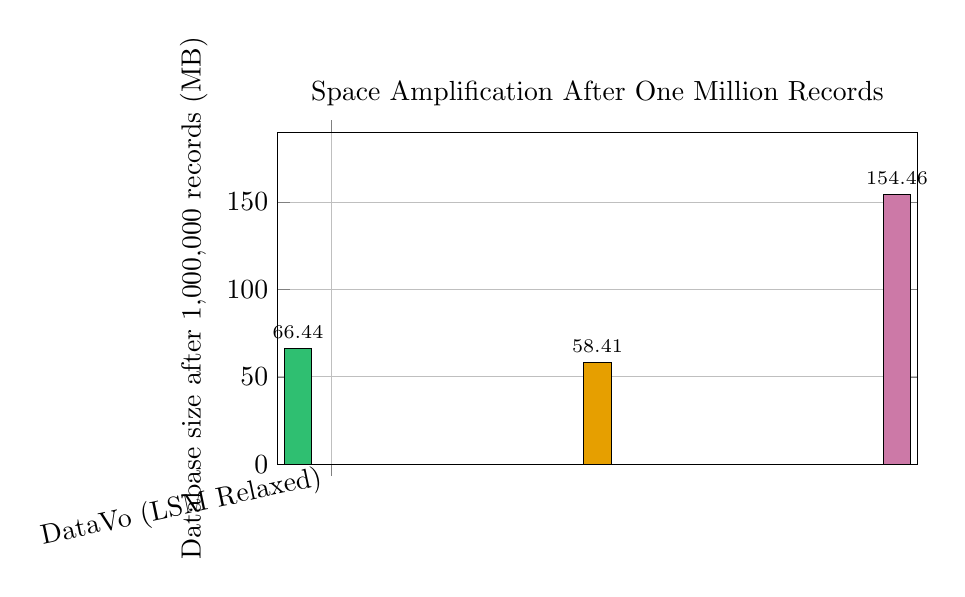
\begin{tikzpicture}
\begin{axis}[
    ybar,
    width=0.8\linewidth,
    height=5.8cm,
    ylabel={Database size after 1,000,000 records (MB)},
    symbolic x coords={{DataVo (LSM Relaxed)},{SQLite (WAL,normal)},LiteDB},
    xtick=data,
    x tick label style={rotate=12, anchor=east},
    ymin=0,
    ymax=190,
    nodes near coords,
    nodes near coords align={vertical},
    every node near coord/.append style={font=\scriptsize},
    grid=major,
    title={Space Amplification After One Million Records},
]
\addplot[fill=datavoFreshGreen] coordinates {({DataVo (LSM Relaxed)},66.443)};
\addplot[fill=sqliteOrange] coordinates {({SQLite (WAL,normal)},58.405)};
\addplot[fill=liteDbPink] coordinates {(LiteDB,154.461)};
\end{axis}
\end{tikzpicture}
}
\end{center}

% Figure 2: Vector Search Latency vs Allocation Double-Axis Bar
\begin{center}
\resizebox{\linewidth}{!}{%
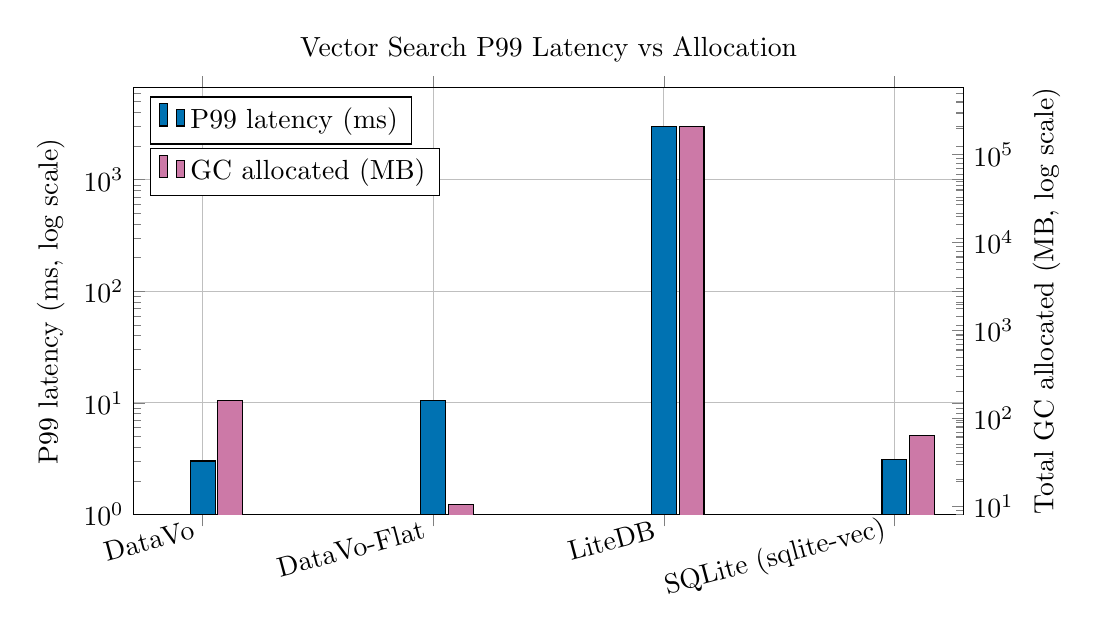
\begin{tikzpicture}
\begin{axis}[
    width=\linewidth,
    height=7.0cm,
    ymode=log,
    ylabel={P99 latency (ms, log scale)},
    symbolic x coords={DataVo,{DataVo-Flat},LiteDB,{SQLite (sqlite-vec)}},
    xtick=data,
    x tick label style={rotate=15, anchor=east},
    ybar,
    bar width=9pt,
    ymin=1,
    title={Vector Search P99 Latency vs Allocation},
    legend style={at={(0.02,0.98)},anchor=north west},
    grid=major,
]
\addplot[fill=datavoBlue] coordinates {
    (DataVo,3.015500)
    ({DataVo-Flat},10.488584)
    (LiteDB,2989.564083)
    ({SQLite (sqlite-vec)},3.106291)
};
\addlegendentry{P99 latency (ms)}
\end{axis}
\begin{axis}[
    width=\linewidth,
    height=7.0cm,
    axis y line*=right,
    axis x line=none,
    ymode=log,
    ylabel={Total GC allocated (MB, log scale)},
    symbolic x coords={DataVo,{DataVo-Flat},LiteDB,{SQLite (sqlite-vec)}},
    xtick=data,
    ybar,
    bar width=9pt,
    bar shift=10pt,
    ymin=8,
    legend style={at={(0.02,0.86)},anchor=north west},
]
\addplot[fill=liteDbPink] coordinates {
    (DataVo,157.246)
    ({DataVo-Flat},10.331)
    (LiteDB,208915.002)
    ({SQLite (sqlite-vec)},63.427)
};
\addlegendentry{GC allocated (MB)}
\end{axis}
\end{tikzpicture}
}
\end{center}

% Figure 3: Concurrent Operations Throughput OPS Comparison
\begin{center}
\resizebox{0.8\linewidth}{!}{%
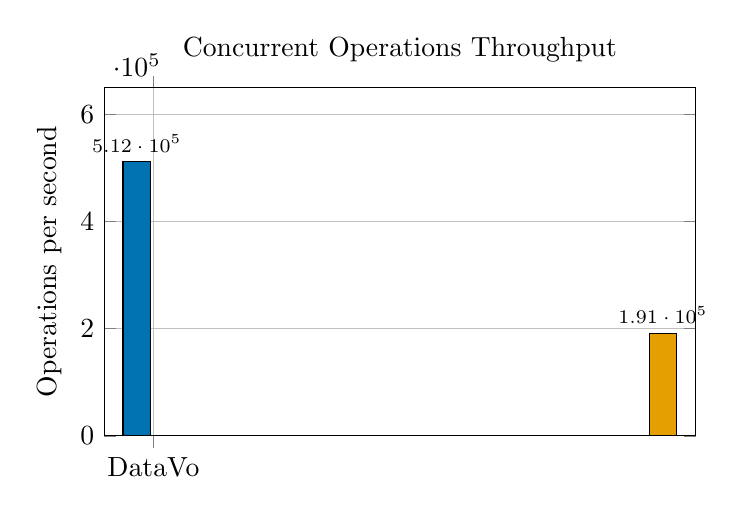
\begin{tikzpicture}
\begin{axis}[
    ybar,
    width=0.75\linewidth,
    height=6.0cm,
    ylabel={Operations per second},
    symbolic x coords={DataVo,SQLite},
    xtick=data,
    ymin=0,
    ymax=650000,
    nodes near coords,
    nodes near coords align={vertical},
    every node near coord/.append style={font=\scriptsize},
    grid=major,
    title={Concurrent Operations Throughput},
]
\addplot[fill=datavoBlue] coordinates {(DataVo,511827.704)};
\addplot[fill=sqliteOrange] coordinates {(SQLite,191068.481)};
\end{axis}
\end{tikzpicture}
}
\end{center}
